%!TEX root = ../template.tex
%%%%%%%%%%%%%%%%%%%%%%%%%%%%%%%%%%%%%%%%%%%%%%%%%%%%%%%%%%%%%%%%%%%%
%% chapter3.tex
%% NOVA thesis document file
%%
%% Chapter with a short latex tutorial and examples
%%%%%%%%%%%%%%%%%%%%%%%%%%%%%%%%%%%%%%%%%%%%%%%%%%%%%%%%%%%%%%%%%%%%

\typeout{NT FILE chapter3.tex}%

\makeatletter
\newcommand{\ntifpkgloaded}{%
  \@ifpackageloaded%
}
\makeatother

\chapter{State-Of-The-Art}
\label{cha:state_of_the_art}


\section{Ultrasound Transducers}
\label{sec:ultrasound_transducers}

\subsection{Ultrasound Transducer Materials}
\label{subsec:ultrasound_trasnducer_materials}

It is impossible to establish a review of existing ultrasound imaging (USI) and ultrasound stimulation (USS) systems without first highlighting the current materials used to implement the ultrasound transducers (USTs). The choice of material impacts frequency range, transducing power efficiency, biocompatibility, the architecture of the interfacing electronics and thus the cost of high-volume manufacturing of the trasnducers, the interfacing electronic system and the integration of the former with the latter. Due to their miniaturisation, moderate-to-high centre frequency range and moderate-to-high electromechanical transducing efficiency (resulting in lower driving power dissipation) capabilities, this sub-section focuses on the review of the benefits and limitations of UST implemented using bulk piezoelectric materials, piezoelectric micromachined ultrasound transducers (PMUTs) and capacitive micromachined ultrasound transducers (CMUTs) - transducing materials dominant in medical applications. Notice that bulk piezoelectric and PMUTs both use piezoelectric materials for implementing the UST, but differ in manufacturing process, geometry and transducer electromechanical coefficients - affecting also their equivalent electric model used upon the development of the interfacing electronics.

Modern bulk piezoelectric transducer materials have the advantage of exhibiting moderate-to-high electromechanical coupling coefficients while presenting high quality factors. Lead zirconate titanate (PZT), a ceramic-based piezoelectric material, and lead magnesium niobate-lead titanate (PMN-PT), a relaxor ferroelectric-based piezoelectric material, have been widely adopted in recent years due to their electromechanical properties enabling the miniaturisation and compact integration 
of the transducers with the interfacing electronics while still providing for a whide range of existing and emerging medical applications \cite{https://iopscience.iop.org/article/10.1088/1361-6463/ac8687}. 

Bulk PZT transducer materials present thickness-mode electromechanical coupling coefficients 
($k_{33}$) typically ranging from 0.5 to 0.75, while presenting mechanical 
quality factors ($Q_m$) ranging between 30 and 80 at a high acoustic impedance 
typically found within 33 to 35 MRayl \cite{https://link.springer.com/book/10.1007/978-0-387-76540-2 Fig 10.12} 
\cite{https://iopscience.iop.org/article/10.1088/1361-6463/ac8687}.
The presented coupling coefficient enable a lower driving power when 
aiming for high-intensity focal spot profiles. Due to its high acoustic impedance, 
PZT transducers require matching layers to minimize acoustic 
energy losses associated to the impedance mismatch between the human body 
and the transducer to improve the efficiency and efficacy of the 
US therapeutic system \cite{https://pubmed.ncbi.nlm.nih.gov/32708159/} \cite{https://www.nature.com/articles/srep42863}.
While theurapeutic applications profit from high $Q_m$, resulting in narrow-band, 
long response time transducers to maximize energy transmitted versus 
provided driving stimuli, diagnostic applications require broad-band, 
short impulse response transducers featuring low $Q_m$ to maximize the 
lateral resolution of the reconstructed US image. As such, for diagnostic 
applications PZT transducers require a mechanical or electrical mechanism to lower 
their $Q_m$ \cite{}\cite{}. Damping backing layers have been explored 
in the context of US applications capable of diagnostic and therapeutic operation modes \cite{}. 
However, this mechanical approach renders the backed transducers ineffective 
for the transmission of high-intensity focused US beams, and transducer arrays 
must feature a configuration of diagnostic and therapeutic-optimised transducers 
that usually compromises on the diagnostic capabilities of the system 
\cite{Hassan Random distribution}\cite{Chao Chen Cross}.
Electronic feedback systems have been recently started to be explored 
in the context of electrically lowering the $Q_m$ factor of the transducer 
when operating in diagnostic (imaging) mode \cite{https://ieeexplore.ieee.org/document/8589657}.
By coupling an electrical resonator with a low quality factor to the transducer with a 
high quality factor, the latter can be lowered by controlling 
the strength of the coupling between both resonators. Increasing the 
amplitude of the electrical resonator's output will lead to 
a lower quality factor for the transducer, enabling it 
to maintain optimal impulse response in both therapeutic and diagnostic 
applications. This is a very recent and active research track, and 
it is being actively pursued at the research.

Similar to PZT, PMN-PT also experiences significant acoustic impedance mismatch 
and acoustic energy losses when being interfaced with human tissue, due to its 
high acoustic impedance ranging from 35 to 40 MRayl depending 
on the percentage of lead titanate (PT) present in the composite \cite{https://pubmed.ncbi.nlm.nih.gov/32708159/}.
PMN-PT transducers also feature a high $Q_m$ in the same order of magnitude as that of PZT, ranging from 150 to 180, 
needing to be compensated for when aiming for their usage on US diagnostic applications as well.
However, the electromechanical coupling coefficient of PMN-PT ranges from 0.85 up to 0.95, providing 
for a lower required driving power to achieve similar focal spot intensities when compared to PZT transducers. Additionally, 
the higher coupling coefficient of PMN-PT transducers also enables for an higher sensitivity, meaning that 
a similar strain force stimuli can generate a greater charge displacement when compared to PZT, and thus 
an higher voltage signal can be read by the interfacing electronics in diagnostic applications, relaxing their 
input referred noise requirements and reducing their area and power dissipation requirements \cite{https://iopscience.iop.org/article/10.1088/1361-6463/ac8687}.

The Curie point of a piezoelectric materials is the temperature at which the 
piezoelectricity properties are permanently altered from its original 
conditions, and in general, piezoelectric materials lose the ability of 
charge-displacement past this point \cite{https://iopscience.iop.org/article/10.1088/1361-6463/ac8687}.
The development of suitable manufacturing and integration procedures of piezoelectric 
transducer arrays that do not change their underlying physical properties is, as such, 
an active research field and crucial for the pursuit of evermore miniaturised and 
energy efficient US-based systems and their applications. PZT presents an higher 
Curie temperature (350 °C) than that of PMN-PT (130 °C–170 °C), introducing significant 
challenges in the fabrication of PMN-PT devices, as well as transferring the material onto 
backing substrates without damage. This introduces harsh limitations on the range of 
applications of PMN-PT. The electromechanical transducing capabilities of PMN-PT 
come at the expense of an increased complexity regarding the manufacturing and 
integration process of the transducer arrays when compared to PZT 
\cite{https://doi.org/10.1533/9781845699758.1.318, https://iopscience.iop.org/article/10.1088/1361-6463/ac8687}. 
Another great advantage of PMN-PT-based transducers is tied to its DC-bias sensitiveness. Some US transducers provide a acoustic to electric transduction sensitivity that depends on the DC-bias voltage level between both electrode plates of the transducer. Example of this phenomena are CMUTs and PMN-PT or PIN-PMN-PT based transducers. More specifically, bulk PMN-PT transducers only exhibit electromechanical conversion capability while a bias voltage is applied, and it has been verified that an inversion of the DC-bias level introduces a 90 $\mathrm{^\circ}$ phase shift in the received or transmitted US waves relative to a forward-biased transducer \cite{10.1109/ULTSYM.2016.7728854, 10.1109/ULTSYM.2018.8579821}. This effect has been successfully explored to enable the implementation of an electronically-reconfigurable acoustic Fresnel Lens paving new unexplored research paths towards the miniaturisation and reduction of the power dissipation of imaging/HIFU-capable US row-column transducer array applications \cite{10.1109/ULTSYM.2018.8579821, 10.1109/ULTSYM.2018.8579821, 10.1109/ULTSYM.2019.8926257}.

Both previously discussed transducer materials contain lead, which can lead to significant 
environmental damage when the devices are improperly disposed off \cite{https://iopscience.iop.org/article/10.1088/1361-6463/ac8687, 
https://doi.org/10.1533/9781845699758.1.318, https://doi.org/10.1016/j.ceramint.2021.03.054}. 
Additionally, although not well understood, existing concerns have lead recent studies regarding the biocompatibility of using lead-based materials 
in medical implantable devices that are placed in direct contact with the patient's tissue. Lead is a toxic heavy metal that can lead to significant health complications of patients when their body tissue comes into contact with the lead-based material for long periods of time, 
resulting in a growing research effort to implement lead-free ultrasound transducer materials \cite{https://doi.org/10.1016/j.ceramint.2021.03.054, https://iopscience.iop.org/article/10.1088/1361-6463/ac8687}. Polymer-based, lead-free transducer materials have emerged as a promising alternative to PZT and PMN-PT 
based piezoelectric materials, offering greater biocompatibility and less environmental damage risk 
\cite{https://iopscience.iop.org/article/10.1088/1361-6463/ac8687}. 
Polymer-based piezoelectric materials such as polyvinylidene fluoride (PVDF), 
barium titanate (BaTiO3) and potassium sodium niobate (KNN) have emerged as potential replacement 
for lead-based ceramic composite piezoelectric materials.
Compared to lead-based bulk piezoelectric materials 
(presenting a brittle texture due to their composite ceramic matrix lattice), 
polymer piezoelectric materials are flexible and lightweight, while enabling a 
wider range of manufacturing processes in different substrates, presenting lesser 
complexity manufacturing and electronic integration of transducer arrays 
\cite{https://doi.org/10.1016/j.ceramint.2021.03.054}. As an example, PVDF provides an acoustic impedance 
ranging from 4-10 MRayl, being closer to that of human-tissue \cite{https://ieeexplore.ieee.org/abstract/document/9354791}. 
In the scope of biomedical applications, 
the increased flexibility lowers the acoustic impedance of the transducer, offering a greater 
conformability and lower acoustic impedance mismatch towards human tissue - increasing the efficiency 
of acoustic energy transfer between the human body and the transducer, making them specially suitable for 
US diagnostic applications \cite{https://doi.org/10.1016/j.ceramint.2021.03.054}. 
While still requiring matching layers to maximise the mechanical energy transfer between the 
transducer and human body, the lower transducer array manufacturing and integration complexity also increases the yield 
of transducer elements within the large-area transducer arrays, which is currently an important challenge 
in transducer arrays employing bulk lead-based piezoelectric materials containing >1000 elements 
\cite{https://www.nature.com/articles/s41467-024-47074-1}. 
However, the increased flexibility, decreased manufacturing and integration complexity and increased 
biocompatibility of polymer-based piezoelectric transducer materials comes at the expense of 
lower electromechanical coupling and charge displacement coefficients \cite{https://doi.org/10.1016/j.ceramint.2021.03.054}.
Despite presenting the highest piezoelectricity performance among piezoelectric polymers, PVDF 
presents an electromechanical coupling coefficient ranging from 0.2 to 0.5 in stacked PVDF-based composite materials
\cite{https://doi.org/10.1016/j.jmbbm.2021.104669, https://doi.org/10.1002/adfm.201908724, https://doi.org/10.1007/978-0-387-76540-2_7}. 
Compared to PZT or PMN-PT-based paterials, the reduced electromechanical coupling coefficient of polymer-based 
piezoelectric materials can lead to a doubling of the power dissipation of the driving electronics 
in therapeutic US applications. The additional power disspation reduces the portability 
of the therapeutic device and, in some cases, can lead to a violation of FDA guidelines 
regarding the maximum power of 0.5 W to prevent the uncontrolled temperature increase of human tissue, 
rendering polymer-based piezoelectric materials unsuitable for the design of US stimulation devices \cite{Fomenko2018, Dalecki2004}.

\begin{figure}
  \centering
  \begin{subfigure}[][][t]{0.3\textwidth}
      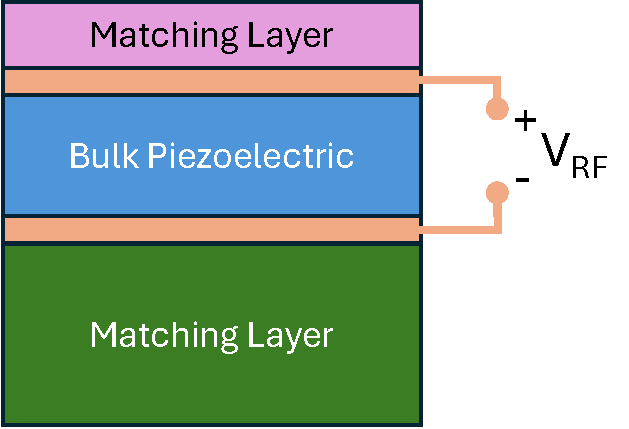
\includegraphics[width=0.45\textwidth]{Chapters/Figures/Ch2_UltrasoundFundamentals/bulk_piezoelectric.pdf}
      \label{fig:ch3_bulk_piezo}
  \end{subfigure}
  %\hfill
  \begin{subfigure}[][][b]{0.3\textwidth}
      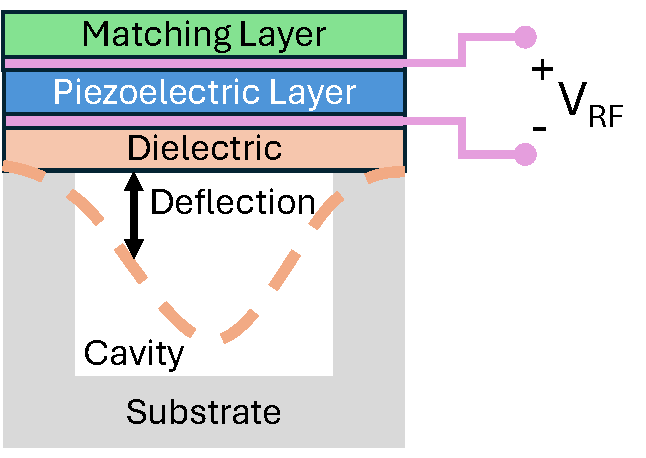
\includegraphics[width=0.45\textwidth]{Chapters/Figures/Ch2_UltrasoundFundamentals/pmut.pdf}
      \label{fig:ch3_pmut}
  \end{subfigure}
  %\hfill
  \begin{subfigure}[][][b]{0.3\textwidth}
      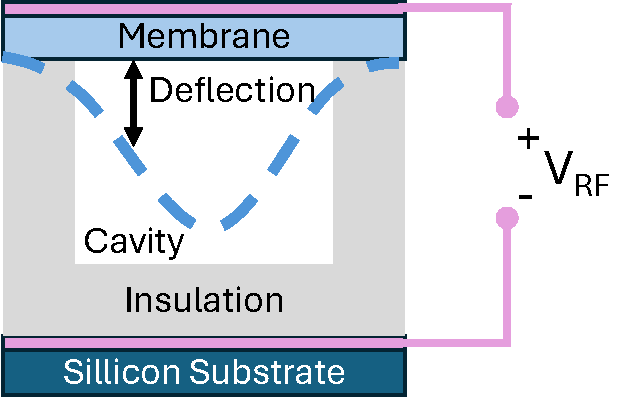
\includegraphics[width=0.45\textwidth]{Chapters/Figures/Ch2_UltrasoundFundamentals/cmut.pdf}
      \label{fig:ch3_cmut}
  \end{subfigure}

  \caption{Creating subfigures in \LaTeX.}
  \label{fig:ch3_transducer_types}
\end{figure}

The last two classes of transducer discussed in this section, PMUTs and CMUTs, consist of material 
membranes micromachined to a few micron-level thickness, enabling the softened materials 
to mechanically interact with US pressure waves with significantly lower acoustic impedance, 
working on the principle of the flexural vibration of a thin membrane film.
The differences between PMUTs and CMUTs lie on the physical phenomena governing the 
transduction between electrical sigals and the mechanical displacement of the 
membrane \cite{https://doi.org/10.1109/ACCESS.2024.3359906}.
In general, the enhanced acoustic impedance matching removes the need for matching layers when 
interfacing the transducer with soft tissue, consequently decreasing the complexity of transducer 
integration processes \cite{https://doi.org/10.1038/s41378-023-00555-7, https://doi.org/10.1109/TUFFC.2021.3112917}. 
PMUTs are micromembrane ultrasound transducers exhibiting thin-film piezoelectricity, 
backed by an acoustic cavity and encapsulated between two flexible metal electrode layers.
PZT (lead-based), PVDF and more recently aluminium nitride (AIN) (lead-free alternatives to PZT) are amongst the most widely 
adopted PMUT materials, and the lower acoustic impedance reduces the quality factor of the transducers, 
increasing their bandwidth and consequently axial resolution of obtained US images - making PMUTs especially 
suitable for US diagnostic applications \cite{https://doi.org/10.1109/ACCESS.2024.3359906, 10.1109/TRANSDUCERS.2019.8808774, 10.1109/ULTSYM.2019.8926015}.
PMUT transducers are still operated in its poling direction (3-3 electromechanical coupling mode), 
but the significantly lower thickness geometry significantly changes the electromechanical properties of the piezoelectric material 
when compared to its bulk transducer material counterpart, and together with the air-backing cavity 
provide for low quality factor, wide-bandwidth transducer suitable for diagnostic applications. 
The electromechanical coupling coefficient of PMUTs is significantly lower when compared to bulk 
PMN-PT transducers, making them less suitable for power-efficient, portable, 
miniaturised US therapeutic applications \cite{https://www.nature.com/articles/s41378-024-00783-5, https://doi.org/10.1038/s41378-023-00555-7}.

The basic operational principle of CMUTs relies on the change of capacitance while the transducer mechanically 
interacts with US waves. CMUTs are implemented in a sillicon substrate, using a flexural membrane consisting 
of a metal electrode and a flexural micromachined dielectric substrate supported by an insulator \cite{https://doi.org/10.1109/TUFFC.2021.3112917}. 
This membrane is suspended over a cavity acting as an air-backing matching layer providing, similarly to PMUTs, 
significant transducer bandwidth and axial resolution improvements - making CMUTs especially suitable for US 
diagnostic applications \cite{https://doi.org/10.1016/j.jmu.2012.02.001, 10.1109/ACCESS.2024.3359906}. 
The substrate is then integrated on top of the bottom electrode pad. The 
US pressure wave-induced mechanical displacement of the insulated top electrode provides for capacitance 
changes relative to bottom electrode. These capacitance changes are then transduced into electrical signals 
with an energy directly proportional to the energy of the sensed mechanical waves. 
Applying an AC electrical signal between the top and bottom electrodes charges/discharges the 
equivalent capacitor of the CMUT transducer, leading also to the mechanical displacement of the suspended membrane relative to the susbtrate, enabling also the 
transmission of US waves. The sillicon substrate integration of CMUTs enables the utilization of 
fabrication methods are easily integrated into a CMOS manufacturing process, making the low transducer array manufacturing and integration complexity the main advantage of CMUTs \cite{10.1109/TUFFC.2021.3112917, 10.1109/ACCESS.2024.3359906, https://www.nature.com/articles/s41378-024-00783-5}. However, while the low quality factor of CMUTs provides suitability towards US medical imaging devices, the low electromechnaical coupling coefficient renders CMUTs not suitable for US wave transmission due to the high driving power required by CMUTs to achieve moderate-to-high intensity focal spot pressures required by therapeutic applications \cite{10.1109/TUFFC.2021.3112917, 10.1109/ULTSYM.2012.0020}.

% TODO: Table with the description of the material properties of the most commonly 
% utilized materials for biomedical applications.

\subsection{Ultrasound Transducer Array Integration Methods}
\label{subsec:ultrasound_transducer_system_integration}


\begin{figure}[ht]
  \centering
  \includegraphics[width=\textwidth]{Chapters/Figures/target_fUSVNS.png}
  \label{fig:asic_sensor_integration}
\end{figure}

Achieving a miniaturized ultrasound 3D imaging system requires the compact integration of the two fundamental components of the system - an ultrasound transducer matrix and the interfacing integrated electronics. Three main methods can be used to achieve this integration (Fig. \ref{fig:asic_sensor_integration}). 
\par
The highest integration possible is achieved through the use of \textit{monolithic integration} (Fig. \ref{fig:monolithic_integration}). Regarding the integration of bulk piezoelectric transducers, an initial commercially available slab of transducer material is diced to the total width and length composing the total aperture of the transducer array. A first sub-dicing procedure cutting from 20\% to 60\% of the total thickness of the diced slab is then performed in both longitudinal and transversal directions to delimit each column and row, respectively, of the transducer matrix. The sub-diced slab is then flipped and aligned with the respective pads reaching from the top-most layer of the CMOS technology metal stack. The bonding is most commonly performed through the use of a chemical bonding process, where a conductive adhesive epoxy is cured at a temperature low enough to not surpass the Curie point of the transducer while still allowing for a strong bond. An alternative to the use of conductive epoxy is the use of an anisotropic conductive film (ACF) applied directly to the CMOS chip. After curing, a final sub-dicing through the rows and columns is applied to finally separate each transducer pillar, finally filling the kerf sections with a non-conductive epoxy to increase the durability of the micron-scale apparatus. To prevent damage of the CMOS chip in this final dicing procedure, a sacrificial epoxy layer is added, finalizing with the introduction of a conductive sheet establishing the virtual ground (common potential) in the top plate of every transducer pillar (Fig. \ref{fig:monolithic_integration}) \cite{TiagoCosta2018}. 
Monolithic integration has several important advantages compared to other alternatives. The direct bonding between the trasnducer and the top-level metal layer of the CMOS technology stack allows for the optimal minimization of the electric parasitic passive components that are known to alter the impulse response of the transducer \cite{}. More specifically, from the point-of-view of a therapy-oriented device design, the minimization of the parasitic capacitance in the ASIC-to-transducer optimizes the power transfer between the HV driving electronics and the transducer matrix, consequently enabling for maximum power delivered at the beamformed focal spot \cite{TiacoCosta2018, HassanTiago2022}. Conversely, without proper control and empirical optimization of the curing time for the bonding conductive adhesive layer, and an incorrect choice of the cutting depth in each sub-dicing procedure, the yield of each successfully integrated transducer pillar with each respective pad can become exceedingly low with pillars being broken out off of their bond and being projected towards the remaining pillars, also destroying them, due to the high rotational speed of the dicing saw (Fig. \ref{fig:low_yield_ghandi}). A yield of 40\% for the totality of the transducer elements of each transducer matrix is settled as the acceptable minimum to consider the transducer matrix capable of operating as an ultrasonic transduction device, and the incorrect calibration of the underlying manufacturing parameters of this integration process can lead to this threshold not being met far too often \cite{}. Moreover, the width of the dicing saw sets the minimum kerf size establishing the physical separation between each transducer element, consequently limiting the minimum pitch achievable with a monolithic integration method. This renders this integration method too restrictive regarding the development of high frequency ultrasound stimulation and imaging systems \cite{}.
\par 
The second integration method addressed in this discussion is \textit{flip-chip bonding} (Fig. \ref{fig:flip_chip_bonding}). 
This technique is most often used in the industry to enable direct integration between CMUTs and the respective CMOS technology \cite{}. Two main types of flip-chip can be discriminated in the literature. An intermediate interposer printed circuit board (PCB) using vias that traverse through the PCB's layers establishing a connection between the transducer elements on the opposite side of the board and the dedicated pads in the top-level metal layer of the CMOS technology stack used for the design of the ASIC (Fig. \ref{fig:through_pcb_via}) \cite{HassanThesisRef182,194}. The second approach replaces the intermediate interposer PCB with a silicon substrate, using a through-(sillicon) substrate via for direct bonding with the transducer elements, in which CMUTs and PMUTs can be directly manufactured in (Fig. \ref{fig:through_silicon_via}) \cite{HassanThesisRef182,193}. Although the use of an intermediate PCB to establish the connection between the transducer elements and each respective pad of the ASIC is a relatively inexpensive method for lower frequency applications, higher frequency applications, where the transducers' pitch is significantly smaller and the size of the required micro-vias for establishing the bonds, leads to a substantial cost increase of the PCB manufacturing process. Moreover, a commonly used fiber-glass based material in PCB manufacturing is fiber-glass flame-retardant epoxy resin (FR-4), presenting a typical dielectric constant of 3.4 \cite{https://www.atlasfibre.com/material/fr-4/, https://link.springer.com/article/10.1007/BF02657420}. The parasitic elements associated with the use of this method lead to a lower power distribution efficiency between the ASIC and each transducer element. On the other hand, a pure sillicon (Si) wafer presents a typical dielectric constant of 11.7, but can vary depending on the oxidation level of its surface \cite{https://iopscience.iop.org/article/10.1088/2053-1591/abf684}. The higher dielectric constant means the use of a through-silicon metal vias can lead to higher integration scale while lowering the effect of parasitics and increasing the power efficiency of a FUS stimulation application. The use of through-wafer vias is a technique currently facilitating the development of high-yield automated manufacturing and integration of CMUT transducer arrays directly with CMOS, which consequently ties this method to a transducer array with lower transmission efficiency compared to bulk piezoelectric transducers, as discussed in the previous section \cite{}. 
Both monolithic and flip-chip integration have been proven as crucial methods to drive the miniaturization of US phased-array-based applications, either for diagnostic or therapeutic applications. The direct accessibility to the bottom plates of each individual transducer element, combined with the use of top-level metal pads within the ASIC's internal active area, is essential to allow cost-effectiveness and efficiency of the miniaturisation of the device. 
\par
Finally, the last method discussed in this section is a \textit{PCB-based} transducer array integration, connecting the ASIC's I/O pads with the transducer array elements using standard PCB design methods and its metal traces to establish a connection to the bottom plate  and wire-bonding for establishing connection to the top plate of the transducer elements (Fig. \ref{fig:pcb_array_integration}). 
The use of a PCB integration method allows for the cheapest option for the interface between the transducer array and the ASIC in a miniaturized US imaging/stimulation solution. However, it comes with several limitations that has led researchers to pursue both of the aforementioned methods. The first limitation, in similarity with a through-substrate via flip-chip bonding solution, is that in higher frequency applications, due to the reduced pitch of US transducer elements, the cost of PCB manufacturing can significantly increase to the customized reduced widths for the interfacing metal tracks that require laser erosion techniques \cite{}. The second limitation is once again tied to the significantly increased parasitics of the PCB board interconnects when compared to the previous methods. In high frequency FUS stimulation or US imaging applications, the incorrect control of the phase-delay the PCB interconnect introduces in the signals due to the transmission line effects of each trace can greatly degrade the quality of the transmitted / received US signal, degrading the efficacy of the application as well. PCB integration is especially useful when interfacing ASICs with 1D transducer arrays. However, throughout the reviewed literature, the main limitation preventing the use of a PCB integration methodology in a matured, highly miniaturised device prototype is the high complexity of interfacing each transducer in a 2D transducer matrix with the I/O pads in the periphery of an ASIC (Fig. \ref{fig:pcb_2d_array_pcb_integration}). The pitch requirements for each micro-via carrying the US signals for the different layers of the PCB layer stack, and the space limitation capping the manufacturing costs of the ASIC, limiting the available I/O pads, quickly drive the costs of the prototype device using this method up while providing for a lower application efficacy when compared to the previous methods. 
\par
What if, when interfacing with a 2D transducer element matrix, to enable a FUS stimulation application through the use of a phased-array, while also allowing for the 3D US imaging of the sonicated medium, only a 1D set of metal interconnects was necessary between the ASIC and each column of the transducer matrix? Would a PCB integration methodology be suitable in that case, when aiming to drive the device prototyping costs down, while avoiding the loss of efficacy and functionality? This was the question asked and successfully answered at the School of Biomedical Engineering, Dalhousie University, Canada, in 2016 \cite{https://ieeexplore.ieee.org/document/7728854, https://ieeexplore.ieee.org/document/8926257, https://ieeexplore.ieee.org/document/9957541}. The use of PMN-PT for the implementation of a crossed row-column transducer enables a DC-bias sensitivity towards the impulse response of each transducer array. By using either a positive or negative HV biasing in the top-plate of each row, a phase shift of $\mathrm{90^\circ}$ or $\mathrm{-90^\circ}$, respectively, is introduced in the transmitted US waves (Fig. \ref{fig:safe_algorithm_imaging}). This Hadamard-encoded electronically programmed phase shift is used to create a Fresnel lens discretized to two binary levels in anti-phase, creating zones of constructive and destructive interference in the sonication medium, ultimately leading to focusing of the transmitted waves in the elevational direction (Fig. \ref{fig:phase_fresnel_lens}). 

%TODO: put equation of fresnel lens element-level phase encoding depending on the elevational angle of focusing. 

The shorted bottom plates of each column of the crossed-electrode array are then used to recover the 3D spatio-temporal information of each 2D slice recovered. Each Hadamard code used to provide set the biasing and the electronically steered Fresnel lens through each row of the crossed-electrode array is ultimately associated with each elevational slice of the sonicated medium, allowing for 3D US images to be recovered while only interfacing with the columns of the array (1D set of metal interconnects). By combining the row-wise bias-encoded Fresnel lens for elevational focusing with a 1D phased array using programmed phased delays in the column-wise US TX pulses for azimuthal focusing, this method effectively enables the use of this crossed electrode configuration for US therapeutic applications (Fig. \ref{fig:safe_algo_therapy}) \cite{https://ieeexplore.ieee.org/document/7728854}.

Regarding the suitability of the crossed-electrode configuration for US diagnostic applications, both main US imaging algorithms, SL and PWC, can be implemented in this crossed-electrode configuration, with the main difference between both implementations being the overall complexity of the PCB integration with the ASIC to allow for reliable US images to be reconstructed. When performing SL imaging, while the shorted bottom electrodes are used to establish the crossed-electrode's column wise 1D phased-array for azimuthal focusing, the shorted row-wise top electrodes are used to established the bias-Hadamard-encoded  Fresnel lens enabling the elevational focusing, creating a FUS scan-line that can be swept across the 3D medium being sonicated. During RX events, the two-way focusing required by SL US imaging can then be achieved by using the reverse beamformed lens used in the column-wise 1D phased array during TX events. However, to mitigate the effect of secondary lobes in the decrease of the reconstructed image's spatial resolution, the RX channels of the US imaging readout system must be connected in the top shorted row-wise crossed electrodes used to establish the bias, leading to a significant increase in PCB integration complexity and a reduction of the miniaturisation form-factor of the device prototype in general. Additionally, the use of wire-bonding techniques to connect the RX channels to the row-wise shorted top electrodes can significantly decrease the signal integrity of the transduced echoes during RX in high-frequency US diagnostic applications, due to the additional parasitic inductance and resistive voltage dividers inherent to the wire-bond. Finally, the use of a HV biasing network in the same interconnect as the low-voltage (LV) RX channel introduces the need to well matched DC biasing networks that can either invalidate the use of a chiplet solution for the US imaging and stimulation-capable device, or introduce the risk of permanent damage to the RX channel integrated electronics leading to the loss of imaging functionality (Fig. \ref{fig:safe_top_electrode_rx_bias}). Alternatively, to mitigate ASIC damaging risks and drive the integration complexity downwards, a PWC imaging method can be used with this crossed-electrode configuration. When performing PWC US imaging, both TX and RX events can be performed using the shorted column-wise bottom electrodes of the array, with the row-wise electrodes being used solemnly for biasing of the bias-sensitive transducer elements, reducing PCB integration complexity without significantly (negatively) affecting the functionality and the reliability of the reconstructed US images. Due to the lack of TX focusing upon the transmission of steered planar/divergent waves, the reception of the echoes can be performed in the same set of 1D electrodes (and focusing direction) as the steered plane-wave TX pulses are transmitted (Fig. \ref{ref:safe_algorithm_planar_wave_imaging}). Secondary lobes can be further mitigated in the digital backend of the data acquisition (DAQ) system by reconstructing the US image using Hadamard-encoded elevational information of each transmitted steered plane wave \cite{https://ieeexplore.ieee.org/document/8926257, https://ieeexplore.ieee.org/document/9957541}.
\par
The previously described technique, designated as \textit{Simultaneous Azimuth and Elevational Compounding} (SAEC), combines planar wave imaging techniques with a PCB integration method dedicated to the integration of electrostrictive transducer elements (PMN-PT) with the interface electronics of the US imaging system \cite{https://ieeexplore.ieee.org/document/9957541}. The use of SAEC reduces the number of interconnections required to interface with a $N\times M$ transducer matrix to $N$ bottom electrode interconnects, facilitating the integration of US diagnostic and therapeutic systems with high-aperture 2D transducer arrays containing > 1000 transducer elements. This does not necessarily impact the power required to drive all the transducer elements of the same column during TX events, once the parasitic capacitances encoding the mechanical losses of each transducer in resonance are added in parallel (Fig. \ref{ref:saec_implications_power}). However,  during RX events, upon the readout of the received US echoes $\times M$ lesser receiver channels are required to enable a reliable reconstruction of the target US image, driving the dissipated power of the system's receiver down  $\times M$, respectively.

Moreover, the use of SAEC places the viability of a PCB integration method on par with monolithic and flip-chip bonding interfaces, with the main advantage of having the possibility for drastically reducing ASIC-array integration costs without the loss of device efficiency and functionality, both in the US diagnostic and therapeutic domains. Finally, while CMOS technologies supporting the integration of HV Bipolar-CMOS-DMOS (BCD) devices for driving the transducer elements are essential for miniaturized systems on chip (SoC) capable of transmitting US waves, the readout of the received echoes can be performed with standard CMOS technologies at a more advanced node that do not necessarily support such BCD devices. Consequently, the use of a PCB integration enables the use of a chiplet solution that can further reduce the total power dissipation of the US image-guided neuromodulation system's receiver, without compromising on the readout signals' integrity.

\section{Transmitting Integrated Circuit Ultrasound Interfaces}
\label{sec:ultrasound_tx_interfaces}

Conventional US systems generate the required HV signals outside of the probe \cite{}. The HV signals would then be applied to each transducer directly, using an interconnection per transducer \cite{}. Driving the miniaturization of US medical devices, while guaranteeing suitable functionality and precise control for increasing the potential of US as a multi-purpose therapeutic and diagnostic technology for true POC solutions, requires the TX functionality to be integrated closer to the US transducer array.  HV switching and multiplexing techniques significantly reduce the amount of interconnections required to drive the TX system. Despite its simplicity and compact integration, multiplexing ultimately limits the frame-rate of an US imaging system, while also diminishing the peak pressure that is possible to be achieved in a FUS system. The time-division-multiplexing (TDM) access of each transducer to its HV driving signal has to be performed at low-to-moderate frequencies (0.5 MHz - 15 MHz) due to the speed limitations of HV BCD technology devices. This inevitably introduces phase errors in the distributed waves, reducing the peak pressure observed in the regions where maximum constructive interference between TX US waves should be observed \cite{}.  Effectively, as it will be discussed in the following subsections, the element-level integration of a TX HV driver is essential for US image-guided neuromodulation  applications, allowing for precise FUS beam-steering while providing for higher imaging resolution US diagnostic systems \cite{beam_steering_tiago_hassan}\cite{milian_tan_pertjis}.

Although it is not the focus of this work, the following subsections discuss recent works achieving compact, wearable and implantable devices capable driving integrated US transducers for both diagnostic and stimulation applications. The discussion will mainly focus on observing the evolution towards higher power efficiency for the transmitting circuits while achieving a lower supply voltage without compromising on the achieved peak pressure sent to the medium. Understanding the limitations and advantages of the transmitting circuits described will enable for a more productive discussion of the power and area specifications that must be imposed on a receiving analog front-end integrated within the same die and/or PCB as the driving circuits.

\subsection{Supporting Semiconductor Technologies}
\label{subsec:supporting_techs}

In Sec. \ref{subsec:ultrasound_trasnducer_materials} it was discussed that in order to achieve sufficient pressure amplitude in the generated US waves in both therapeutic and diagnostic applications, the transducer device requires voltages in the range of 30 V-160 V, depending on the type of transducer material used. Although bulk piezoelectric transducers require the minimum voltage potential observed in the state-of-the-art while still generating enough pressure to achieve intensities close to the required parameters in LIFUS stimulation procedures \cite{TiagoCosta2018}, the required voltage potentials are still far to high for standard CMOS technologies. Previous designs have proposed to generate HV pulses using stacked LV transistors (Fig. \ref{fig:unipolar_hv_driver_topologies_stacked_lv}) \cite{https://ieeexplore.ieee.org/document/6823174}\cite{https://ieeexplore.ieee.org/document/9340356}. However, the increased circuit complexity, potential reliability concerns and the lower switching speed-power efficiency tradeoff this solution offers has led research groups to seek more reliable alternatives.
The amount of charged carriers being distributed to the substrate of standard threshold voltage (standard-VT) (LV) devices can easily trigger a phenomenon known as \textit{latch-up} (Fig. \ref{fig:latch_up}). This phenomenon happens easily if the electric fields have an high enough magnitude that the finite resistance between the doped source contacts and the substrate leads to a positive feedback that eventually \textit{latches} both parasitic bipolar junction transistors (BJT), completely turning them on, and leading to a massive amount of current being drawn from the integrated circuit's supply into the substrate (Fig. \ref{fig:latch_up_positive_feedback}) \cite{RahzaviDesignofAnalogCMOSCircuits2ndEd}.

\begin{figure}[ht]
  \centering
  \includegraphics[width=\textwidth]{Chapters/Figures/target_fUSVNS.png}
  \label{fig:latch_up}
\end{figure}

At the expense of more silicon area to effectively spread out large electrical fields (preventing them from reaching critical values) and consequently increased distances between device terminals, diffusion regions and additional spacing for isolation barriers between the devices, the introduction of a bipolar-CMOS-DMOS\footnote{DMOS: double-diffused metal-oxide-semiconductor technology} (BCD) HV integrated circuit technology (Fig. \ref{fig:bcd_technology}) solves this issue by enabling the co-existence between standard, (low) core-voltage CMOS and HV devices in the same integrated circuit die. Several notable works driving the miniaturization of US HV drivers that are required in wearable US diagnostic and therapy-oriented applications have exploited this technology \cite{works_on_stimulation_US_devices}.

\begin{figure}[ht]
  \centering
  \includegraphics[width=\textwidth]{Chapters/Figures/target_fUSVNS.png}
  \label{fig:bcd_technology}
\end{figure}

\par
In DMOS devices, the source and bulk are connected and aligned with the gate, forming a channel with a length determined by the diffusion between the p-body and the n+ source, rather than the gate's dimensions. The width of the device is typically scaled, not the length. The lightly doped n-well region between the drain and channel acts as a drift region, determining the device’s on-resistance (Ron) and allowing it to handle higher voltages at the drain. DMOS devices are asymmetrical and have limited overdrive, constrained by the gate oxide breakdown voltage (typically around 5–5.5V in TSMC's 180nm BCD technology, being the most commonly observed technology for miniaturized US devices). The gate extends over both the channel and drift region to reduce the electric field along the drift region, though this increases gate capacitance. The HV deep n-well isolates the device’s active parts from the substrate. The lateral structure of the DMOS shows a parasitic BJT formed by the doping profile of the p-body and n-well. To prevent this parasitic transistor from activating, the source and bulk are connected. The n-guard is often connected to a positive voltage to enhance electron collection. Isolation around DMOS devices is achieved with guard rings, whose width and spacing depend on the peak voltage the device needs to handle. However, wider isolation barriers can increase parasitic capacitance and significantly raise the area cost for small transistors. The deep n-well creates a parasitic PNP transistor, which can become forward-biased if the source voltage exceeds the drain, causing hole injection into the substrate. These holes can lead to substrate potential changes, causing dissipation and issues in nearby devices.   To mitigate this, a p-guard ring is used to stabilize the substrate potential, and n-guard rings are also employed to reduce electron injection and latch-up risks. 

%TODO: review the above text.... might need serious re-writting

\subsection{Unipolar Pulsers}
\label{subsec:unipolar_pulsers}

Unipolar pulsers are often referred to as \textit{square-wave pulsers}, and their counter part are the class of \textit{linear-amplifiers}. These are the two main classes allowing for compact integration between TX driver and US transducer. Linear amplifiers can drive the US transducer with a continuous amplitude signal. However, it is enough for most medical US applications to drive the US transducer with discrete-amplitude pulses. Consequently, the higher energy efficiency, reduced die area footprint, and increased bandwidth of pulsers will be the focus of the architectures discussed in this and the following subsection.

\par
Unipolar pulsers implement the functionality of alternate settling of the top plate of the US transducer element towards HV level and ground. Thus, this circuit-level architecture provides the lowest complexity possible for integrated HV US transducer drivers, using a low number of HV devices. The two main topologies observed in the SoTA inverter-based and source-follower (SF)-based HV driver circuit architectures. Both architectures exploit the aforementioned DMOS devices. A common-source (CS) inverter-based, single N-type HV device, is presented in \cite{} to drive the US transducer between HV and ground. The use of a pull-up resistor leads to a significant static power dissipation when the driven top plate of the transducer is pulled to ground. This issue can be mitigated through the use of a complementary P-type HV device to eliminate static power dissipation of the driver.  However, driving the gate of the P-type device requires a level-shifting of the gate-driving signal from 0 V to the $\mathrm{V_{gs}}$  required to close the N-type HV device to a pulsing signal leveled between the HV supply and (HV - $\mathrm{V_{sg}}$) to drive the P-type HV device without introducing reliability issues to the circuit. This has been achieved in \cite{} through the use of a crossed-coupled LV PMOS close to the HV supply to pull the source of the P-type featuring a DC gate-biasing using a supply greater than the supply gate-biasing the N-type HV-devices (Fig. \ref{fig:cross_coupled_inv_based_hv_driver}). This solution introduces possible reliability issues due to the use of LV devices close to the HV supply, although the reference is also shifted towards the mid-level supply biasing the gates of the P-type HV devices. Moreover, the use of three three different HV supply voltages leads to an increased complexity in the layout of the architecture, while observing an increased die area footprint due to the required number of dedicated pads for the supply of the driver. Alternatively, to remove the reliability concerns regarding the use of LV devices in the HV driver, several works have adopted an inverter-based HV driver (half H-bridge topology) architecture using complementary HV devices.  A single driving signal to drive both inverter devices, while using a dedicated pull-up resistor-based level shifter with protection (voltage-clamping) Zener diodes to shift the same driving signal to a suitable range enabling activation of the P-type device (Fig. \ref{fig:level_shifted_inv_based_hv_driver}) \cite{inv_based_1,inv_based_2,inv_based_3, ...}.  The use of a floating ground at the voltage of HVDD–$V_{SG}$ enables the introduction of additional digital driving buffers (cascaded inverters) to increase the settling speed of the HV drivers\cite{}. Latched HV devices have also been observed to increase the switching speed due to the positive feedback the topology introduces in the dynamic of the circuit (Fig. \ref{fig:hv_cross_coupled_drivers})\cite{HassanLatchedHVDriver}. However, careful control of the settling time of each HV gate-driver must be performed to guarantee the HV latches can actually be latched between HVDD and ground. Bulk biasing feedback can be used to both perform settling time delay control and increase the energy efficiency of the driver \cite{}.

\par
Despite the low complexity and power efficiency of the aforementioned solutions, the use of a single-ended unipolar square-wave HV architecture driving the US transducer's top plate between HVDD and ground leads to a great portion of the power dissipation to be related to even-harmonics due to the presence of a DC component in the driving signal (Fig. \ref{fig:second_order_hamronics_leakage}) \cite{}. This spectral power leakage associated to distortion components of the square wave diminish the SNR of a US imaging being reconstructed using such a TX driving pulse (Fig. \ref{fig:second_order_hamronics_leakage}) \cite{}. It also renders this driving method not suitable for other imaging techniques such as second-order tissue harmonic imaging \cite{}, pulse inversion \cite{} and chirp encoding \cite{}. At the expense of  $4\times$ increase in power dissipation, the use of a bipolar, symmetric square-wave driving the top-plate of the US transducer between HVDD and HVSS, with $\mathrm{HVSS = -HVDD}$, removes the signal's DC component (Fig. \ref{fig:bipolar_hv_pulser}), therefore mitigating this disadvantage.  The two most prominent bipolar pulser architectures found within the literature are the HV source-follower (SF) and the inverter-based driver. While an inverter-based topology offers superior energy efficiency at moderate-to-higher central frequencies \cite{InverterBasedBipolarDriver-https://ieeexplore.ieee.org/document/9365808}, the SF enables greater settling speeds at the expense of a greater architectrual complexity, being suitable for high-frequency imaging and FUS applications \cite{SourceFollowerBipolarDriver-https://ieeexplore.ieee.org/document/8747466}. 
%Finally, the use of integrated full H-bridge drivers have been previously explored for tissue-electrode excitation \cite{}, and are currently under active research in the Bioelectronics Group of TU Delft for their integration in US FUS systems (Fig. \ref{fig:hv_h_bridge_driver}).

\subsection{Multi-Level Pulsers}
\label{subsec:multilevel_pulsers}

Multi-level pulsers have become critical for next generation US HV pulsers. Apodization modulates the system response of the transducer element, enabling the concentration of the transmitted mechanical energy in the main lobe of the transmitted FUS wave \cite{SzaboElementApodization}. As such, for SL imaging applications, the use of a multi-level pulsers allows for transducer element-level temporal and spatial apodization (Fig. \ref{fig:temporal_spatial_apodization}) that leads to significant spatial resolution improvement by reducing the side-lobe magnitude (Fig. \ref{fig:side_lobe_reduction}). The use of a multi-level pulsed wave to approximate a sinusoidal, continuous transmitting wave enables for a significant increase in the linearity of the received US echo due to the concentration of the energy in the main lobe, leading to an increased SNR for the reconstructed image \cite{SzaboSpatialResolutionImage}. Regarding stimulation applications, this spatial and temporal apodization leading to the concentration of the mechanical energy in the main lobe of transmitted FUS beam leads to an increase efficacy for the therapy application while improving spatial resolution of the highest pressure region of the generated focal spot \cite{}. Furthermore, although the generation of a multi-level pulsed wave inevitably requires an increase in hardware complexity,  it has also been observed that significantly improves the energy efficiency of the HV drivers in two different ways. On one hand, upon the discharging of the transducer's parasitic capacitor (associated with its mechanical losses) between consecutive supply levels, the removed charge can be recycled back into the respective HV supply, leading to power dissipation reduction up to ~40\% \cite{ChaoChenReviewPaperRef38}. On the other hand, it has been observed that the contribution of each individual element in a phased-array exciting each element of an US transducer matrix is different and dependant on the relative position of each element to the focal spot generated through the transmition of a FUS wave \cite{MasoumehIUSPublication,AssociatiedRefs}. Thus, scaling the amplitude of the excitation pulse of each individual element to its contribution to the focal-spot's peak pressure leads to a significant reduction in the total power dissipation of the ASIC, while leading to minimal losses in pressure at the intended focal-spot's volumetric region (Fig. \ref{masoumeh_scaled_voltage_contributions}). 


\begin{equation}
    \label{eq:charge_unipolar_driver}
    Q_{UP} = C_p \ (HVDD - 0  \ V) = C_p \ HVDD \ [C]
\end{equation}

\begin{equation}
    \label{eq:charge_recycling_multi_level_driver}
    Q_{MP} = C_p \ \left( N \cdot \frac{HVDD}{N-1} - (N-1)\cdot \frac{HVDD}{N-1}\right) = C_p \frac{HVDD}{N-1} \ [C]
\end{equation}

Where $C_p$ is the parasitic capacitance of the US transducer element.
\\
\par 
The concept behind charge recycling in $\mathrm{N-level}$ pulsers is demonstrated in Fig. \ref{fig:n_level_charge_recycling_drivers}. $N-1$ HV switches are used to charge and discharge the US trasnducer element between consecutive HV levels by connecting the top-plate of the trasnducer each respective supply. Compared to a unipolar HV driver, where the transducer's parasitic capacitance is completely discharged to ground in each cycle (\ref{eq:charge_unipolar_driver}), in a step-wise downward transition, a $1/(N-1)$ fraction of the total charge being discharged from the transducer is recycled back to the lower regulated supply (\ref{eq:charge_recycling_multi_level_driver}) \cite{ChaoChenReviewPaperRef38}. 
Consequently, the dynamic power dissipation (\ref{eq:power_dissipation_cap}) of multi-level pulsers with N levels is reduced by a factor of $(N-1)$ (\ref{eq:dynamic_power_dissipation_reduction}). 

\begin{equation}
    \label{eq:power_dissipation_cap}
    P_D = f_{0}  \ C_p \ V^2 \ [W]
\end{equation}
\begin{equation}
    \label{eq:dynamic_power_dissipation_reduction}
    f_0 \ C_p \ HVDD^2 \longrightarrow f_0 \ C_p \ HVDD \cdot \frac{HVDD}{N-1}
\end{equation}
Where $f_0$ is the cycle frequency driving each step of the pulse.
\\
N-level pulsers require multiple HV supply voltages distributed off-chip, reducing the integration level of a miniaturised US stimulation ASIC due the increase number of supply pads and die area. Moreover, the additional power dissipation upon driving the HV switches to connect individual transducer elements to each available HV supply counter-balances the energy efficiency increase through the use of this driving architecture. To address these issues, multiple schemes tackling the increased hardware complexity of this method have been proposed \cite{ref1,ref2,ref3,...}.  Instead of switching both transducer electrodes to ground, the use of an HV switch in parallel with a PMUT transducer has been used to short-circuit the trasnducer's plates creating a virtual ground in the driving pulse signal, while the bipolar pulser drives the top-plate of the transducer element between symmetric HVDD supplies \cite{}. This method has the main disadvantage of being suitable for transducer materials exploiting the 31 oscillation mode for generating the US mechanical waves, namely CMUTs and PMUT, once these materials enable a low complexity integration and access between both of the transducer's plate electrodes and the ASIC (Fig. \ref{fig:cmuts}, \ref{fig:pmuts}). In bulk piezoelectric transducers, the bottom electrode of the transducer element is vertically opposed to the ASIC, and must rely on a high-complexity, dedicated wire-bond interconnection to allow for its access (Fig. \ref{fig:bulk}).  
Other works targeting the increased hardware complexity of a multi-level pulser capable of more than 3 pulsing levels have used bulky, and often off-chip, stacked-capacitors to generate a multi-level supply \cite{}. HV level-crossing detection using a scaled-down supply of the HV supply and a zero-crossing detector (ZCD) together with a programmable (resistive) ladder to control the charging and discharging of the transducer's top-plate between 7 votlage levels have provided a very compact, pitch-matched solution to a multi-level pulser architecture \cite{}. Finally, the introduction of an inductor per element has also been explored to allow for a $\mathrm{~75\%}$ dynamic power dissipation reduction achieved through charge recycling \cite{https://ieeexplore.ieee.org/abstract/document/9365826, https://ieeexplore.ieee.org/abstract/document/10454286}. At the expense of a significant increase in the form factor of the system, the individual inductors create an LC tank in parallel with the transducer elements being driven at the resonance frequency by the resonant pulser. The energy stored in the magnetic field of the inductor upon the discharging of the transducer can be used to charge it again in the next cycle (Fig. \ref{fig:lc_hv_driver}). The use of an individual inductor per element leads to a prohibitively high form-factor for miniaturised systems capable of driving US trasnducers under a HV regime. To tackle this issue, a single-inductor system has been recently introduced to reuse the energy stored in the passive inductor element with groups of transducer elements in the array at different phases, multiplexing the inductor's stored energy redistribution and achieving $\mathrm{~88\%}$ dynamic power dissipation reduction \cite{https://ieeexplore.ieee.org/document/10904513} (Fig. \ref{fig:single_inductor_hv_driver}).

%TODO: review the circuits and systems being used in electronically steered phased arrays

\section{Receiving Integrated Circuit Ultrasound Interfaces}
\label{sec:ultrasound_tx_interfaces}

Due to propagation-media absorption, scattering and reflection phenomena, the received US echo signal is subjected to a linear-in-dB decay associated to a \textit{propagation dynamic range} ($DR_P$) (Fig. \ref{fig:propagation_dynamic_range}). Moreover, the band-pass characteristic of the transducer element's system response can be modulated through a Gaussian-pulse-modulated cosine in time, leading to an intrinsic \textit{instantaneous dynamic range} ($DR_I$) for the transduced US echoes (Fig. \ref{fig:trasnducer_bandwidth_response}). The first interfacing circuits to the received US echoes are responsible for 1) linear amplification of the transduced US echo, 2) noise and inter-channel electrical correlation suppression to increase the signal's integrity and suppress noise contributions of the following circuits and systems, and 3) time-gain compensation (TGC) of the of the received US echo. The TGC functionality, usually implemented in the analog domain, enables the compression of the high \textit{total dynamic range} ($DR_T = DR_I + DR_P \ [dB]$) of the US echoes to a limited dynamic range relaxing the required specifications of the following circuits and systems in the signal processing chain (Fig. \ref{fig:tgc_total_dynamic_range}).  Alternatively, a channel quantization interfacing exploiting noise-shaping for high-input $DR$ enables direct quantization of the received US echoes without performing TGC in the analog domain \cite{DirectQuantizationSensorToQuantizerWorks}.  The following subsections provide a discussion on the existing architectures establishing the SOTA regarding power, area and noise-efficiency performance employed in miniaturized, integrated diagnostic US systems. The discussion will be mainly guided from a point of view that prefers aggressive miniaturization of the whole analog signal processing chain, reducing it to its core fundamental functionalities. 

\subsection{Low-Noise Amplification}
\label{subsec:sub_array_beamforming_afes}

The low-noise-amplififer (LNA) interfaces directly with the transducer element, providing for a linear amplification of the received US echo, increasing its signal-to-noise-distortion ratio (SNDR) for an enhanced signal integrity upon being processed by the following circuits of the signal processing chain. A secondary variable-gain-amplifier (VGA) cascaded with the LNA is commonly employed to further compress the total dynamic range of the received US echoes through TGC.  
\par
Selecting the correct LNA topology depends, mainly, on the type of US transducer the LNA is interfacing with, the input impedance of the circuits the LNA is driving, and the topology enabling an optimal area, noise and power tradeoff that is specifically tailored for each specific diagnostic application.  The competitive urge to develop LNA with the best noise figure-of-merit (FoM) in relation to the SOTA commonly leads IC designers to over-design their circuits, leading to excessive power dissipation and die-area being used to suppress input-referred noise (IRN) far beyond its required specification. Depending on the center frequency of the TX US waves to achieve the necessary spatial resolution, the total dynamic range of the received US echoes can reach 90 dB  in vascular catheter US probes, due to the elevated attenuation the heart's muscle tissue introduces in the US signal. As such, an higher power dissipation enabling higher IRN suppression capabilities is required \cite{ChaoChen2018,}. On the other hand, the total dynamic range of the US echoes in trans-cutaneous vagus nerve imaging applications is usually within 60-70 dB, relaxing the IRN specification of the employed LNA architecture.  For main LNA architectures can be distinguished throughout the SOTA: 1) voltage amplifiers (VA), usually employed in capacitive feedback configuration, 2) trans-impedance amplifiers (TIA), usually employed in resistive feedback for DC bias-point establishment, 3) current amplifiers (CA), usually employed in capacitive feedback configuration and 4) trans-conductance amplifiers (TCA), usually employed in open-loop (Fig. \ref{fig:lna_topologies}). The output impedance of each transducer material holds a complex relationship between TX driving frequency, material properties, device geometry, the presence of backing and matching layers, and top and bottom electrodes' acoustic impedance. For custom integrated US diagnostic systems, a dedicated characterization of the available US transducer material should be carried out in media applying similar acoustic loads to those verified in the intended diagnostic application \cite{ChaoChenReviewPaper, ChaoChen2018}. Bulk piezoelectric transducers, such as PZT and PMN-PT, and other materials typically employed in PMUTs, feature a relatively low output impedance in resonance (<$\mathrm{2 \ k\Omega}$, leading to the output voltage to be the electrical signal of interest to readout.  Maximizing the signal power transfer between the transducer and the interfacing signal processing chain requires the sensing of the trasnducer's voltage in this case. For this case, VA \cite{} and TCA \cite{} architectures provide a high input impedance through the direct interface between the transducer's signal and input-stage devices' gates, facilitating power and area efficient voltage-sensing. On the other hand, CMUTs and lead-free, polymer-based transducer materials such as PVDF typically feature an high output impedance ($\mathrm{>10 \ k\Omega}$), and their output current is the electrical signal of interest to readout. In this case, the low input impedance CA  \cite{} and TIA \cite{} LNA topologies feature facilitate lower power dissipation and die are footprints when performing current-sensing. 
\par 
Several circuit-level techniques have been employed throughout the SOTA to further optimize power dissipation and the total area of the LNA architecture. Exploiting the duty-cycled TX/RX phase transitions, the use of capacitive negative feedback has been used in VA and CA topologies to improve linearity and remove the noise contribution of the feedback network, at the expense of a greater die are and limited amplifier bandwidth \cite{}. The power-noise efficiency tradeoff has been commonly optimized through the use of a current-reuse (self-biased) inverter-based topology, for the maximization of the LNA's bandwidth under the same DC current biasing point and lower gain error against process-voltage supply-temperature (PVT) variations \cite{}. In general, open-loop LNA topologies have been exploited to minimize the power dissipation and die area FoMs in wide-bandwidth US diagnostic applications, at the expense of an elevated noise floor and decreased linearity \cite{}. For ultra-wide bandwidth (UWB) US diagnostic applications, the incorporation of analog-domain coherent down-conversion-based envelope-detection (ED) has been exploited to greatly increase the power efficiency of the A-mode imaging ASIC \cite{}.  Conversely, despite the increased noise floor and decreased linearity, open-loop amplification topologies are very interesting when aiming to develop a US diagnostic ASIC in advanced CMOS process nodes for further miniaturization of the imaging ASIC. The reduced intrinsic voltage gain of devices in sub 40 nanometer nodes (Fig. \ref{fig:scaling_trends_advanced_process_nodes}) often lead to design choices preferring the use of open-loop inverter-based VA architectures to 1) avoid the increased feedback gain error due to the reduced open-loop gain, 2) achieve sufficiently high output voltage swing and input voltage headroom (mainly avoiding cascode device topologies) while 3) achieving a sufficiently high bandwidth in an energy efficient manner \cite{}.  However, the use of inverter-based amplifier topologies can increase the difficulty of introducing common-mode-feedback (CMFB) circuitry and supply-rail regulation for increased power supply rejection-ratio (PSRR) into the LNA without significantly increasing the power and area per channel of the AFE in general, while decreasing the distortion-free dynamic range \cite{}. 
\par

\subsection{Power Supply Rejection}
\label{subsec:power_supply_rejection_ratio}

Correlated signals, such as digital interference coupled to the analog supply, can be amplified by a factor of N (array size) during averaging, summing or beamforming operations in parallel LNA channels interfacing with closely integrated transducer arrays, potentially causing artifacts in the reconstructed ultrasound image. The correlated noise can lead to an increase in the input-referred noise floor, \cite{Chen2015, Tan2018, Hopf2022},  and even when being below the individual LNA channels' it can still affect image quality (Fig. \ref{fig:lna_noise_contamination}).  Additionally, electrical crosstalk between neighboring LNA channels can elevate side lobes and cause unwanted echoes, requiring careful layout to shield sensitive signals from interference (Fig. \ref{fig:analog_signal_shielding}). A PSRR figure that scales with array size is essential. The single-ended nature of the signals read from US transducers predominantly used in diagnostic US ASICs are most often read out using single-ended LNA architectures to accomodate to the received US echoes while achieving a low power dissipation and area-per-channel FoM \cite{}. The use of current-reuse inverter-amplifiers has been commonly observed in the SOTA. Although their main objective is the increase of power-dissipation efficiency upon the suppression of the IRN figure, it also enables the decoupling of the LNA devices' source nodes from the supply rails \cite{}. The single-ended nature of the current-reuse inverter LNA topologies often employed leads to a relatively inefficient method for increasing the PSRR of the amplifier, once perturbations on the supply rails are directly represented in the single-ended output of the topology.
Dedicated supply low-dropout regulators (LDO) to each LNA sub-array can be used to mitigate the aforementioned issues,. However, the use of a power-intensive LDO for each LNA sub-array prevents significant advances in the power and area-per-channel figures of merit inverter-based LNA AFEs enable (Fig. \ref{fig:supply_regulation_lna}) \cite{Chen2016, Chen2017, Chen2018, Guo2022}. The use of fully differential LNA topologies using common-mode feedback (CMFB) networks decoupling the source-nodes of the amplifier's devices from the supply rails has been identified as a promising method to further increase the PSRR of the amplifier \cite{}. Once again, at the expense of a doubling of the area and power dissipation for each LNA, fully-differential topologies represent any type of signal variations present in the source and gate of the core amplifier's devices, and amplified to the corresponding drain node, in the symmetric output drain node counterpart, leading to a significantly increased PSRR of the differential output signal of the LNA\cite{}.  Finally, the ability of floating inverter amplifiers (FIA) to operate decoupled from the supply rail in their corresponding tracking phase has been identified as a promising way of increasing the PSRR of the associated output (differential) signal in recent years \cite{}. 
\par

\subsection{Time-Gain Compensation (TGC)}
\label{subsec:sub_array_beamforming_afes}

The performance of TGC in the analog domain of the AFE significantly relaxes the IRN specifications of cascaded channel quantization circuits, offering significant power dissipation reduction and miniaturization capabilities for the whole AFE in general \cite{}. Two main methodologies to perform TGC in the analog domain can be discriminated throughout the SOTA. Variable-gain amplifiers (VGAs) apply a continuous, linear-in-dB, amplification to the input signal through time through the means of analog tuning of the DC operating point of the amplifier's core devices \cite{}, and continuous interpolation of discrete gain steps performed using programmable feedback networks \cite{}. 
%TODO: give concrete sota examples

On the other hand, programmable-gain amplifiers (PGAs) perform TGC through the application of linear-in-dB discrete gain-steps to the input US echo signal \cite{}. The use of a digital word to discretely tune the electrical parameters of passive devices can enable a PGA functionality through discrete (resistive) source-degeneration and negative capacitive feedback loop-gain programmability. PGAs offer 
%TODO: give concrete examples

\subsection{Sub-Array Beamforming (µBF) and Channel Multiplexing}
\label{subsec:multiplexed_afes}



\subsection{Channel Quantization}
\label{subsec:on_chip_channel_quantization}

\section{Research Questions}
\label{sec:research_questions}

